\documentclass[../Carre_nights.tex]{subfiles}

\begin{document}

\section{n0348}
\textbf{\Large{The tale of Ibn al-Mansur and the two girls}} \\

\begin{figure}[ht]
\centering
\includegraphics[height=\figsize]{illustrations/volume_4/T04, n0348 - Histoire d’Ibn Al-Mansour avec les deux adolescentes.jpg}
\end{figure}

\textit{\\
"Elle m’offrit la tasse qui était remplie d’eau fraîche parfumée agréablement au musc pur. Moi je la pris et me mis à boire fort lentement et à longs traits en jetant à la dérobée des regards admiratifs à l’adolescente principale, et des regards notoirement reconnaissants à toutes les deux."} \\
—T04, n0348 - Histoire d’Ibn Al-Mansour avec les deux adolescentes \\~\\
\textit{"...she offered me the cup, which was full of clear water, agreeably perfumed with fresh musk, and, taking it, I began to drink very slowly, at the same time sending sidelong glances of admiration at the mistress and open grateful looks at both."} \\
—V02, n0348 - The tale of Ibn al-Mansur and the two girls

\newpage

\section{n0353}
\textbf{\Large{The Tale of Wardan the butcher and the wazir’s daughter}} \\

\begin{figure}[ht]
\centering
\includegraphics[height=\figsize]{illustrations/volume_4/T04, n0353 - Histoire de Wardân le boucher avec la fille du vizir.jpg}
\end{figure}

\textit{\\
"Tous les jours il voyait venir à sa boutique une adolescente splendide de corps et de visage, mais les yeux bien fatigués et aussi les traits bien fatigués et le teint fort pâle. Elle arrivait toujours suivie d’un portefaix chargé de sa hotte..."} \\
—T04, n0353 - Histoire de Wardân le boucher avec la fille du vizir \\~\\
\textit{"Every day a girl of magnificent face and form, but with very tired eyes and pale complexion, would come to his shop, followed by a porter charged with a basket..."} \\
—V02, n0353 - The Tale of Wardan the butcher and the wazir’s daughter

\newpage

\section{n0357}
\textbf{\Large{The tale of Yamlika}} \\

\begin{figure}[ht]
\centering
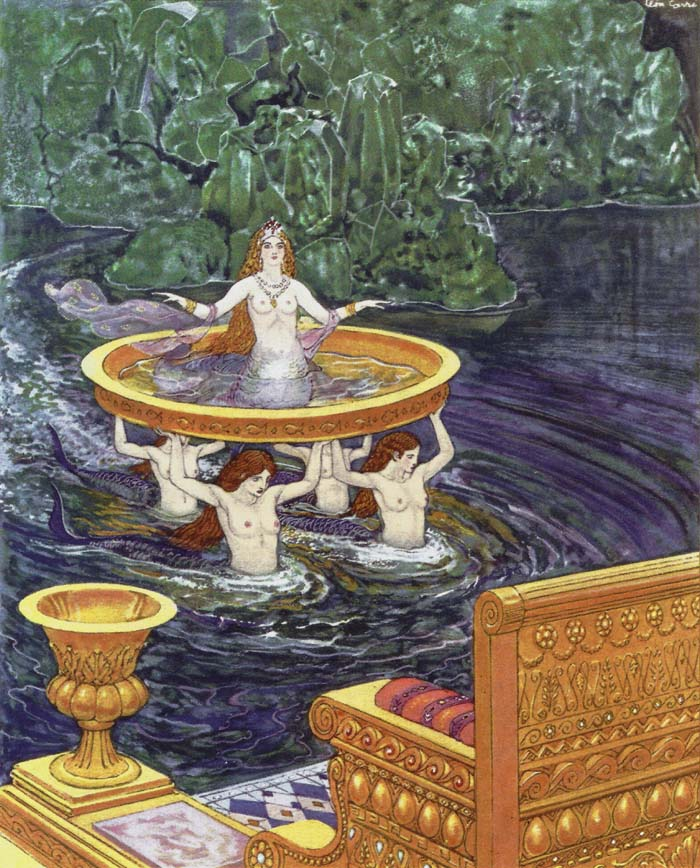
\includegraphics[height=\figsize]{illustrations/volume_4/T04, n0357 - Histoire de la reine Yamlika.jpg}
\end{figure}

\textit{\\
"...apparut de derrière la colline un carré formé par quatre femmes serpentines qui portaient, sur leurs bras élevés au-dessus de leur tête, un grand bassin d’or où se trouvait, souriante et pleine de grâce, la reine."} \\
—T04, n0357 - Histoire de la reine Yamlika \\~\\
\textit{"...four of these snake-women came from behind the hill, gliding in a square and carrying, upon arms upraised above their heads, a vast basin of gold, in which was seated their beautiful smiling Queen."} \\
—V02, n0357 - The tale of Yamlika

\newpage

\section{n0360}
\textbf{\Large{The tale of Yamlika}} \\

\begin{figure}[ht]
\centering
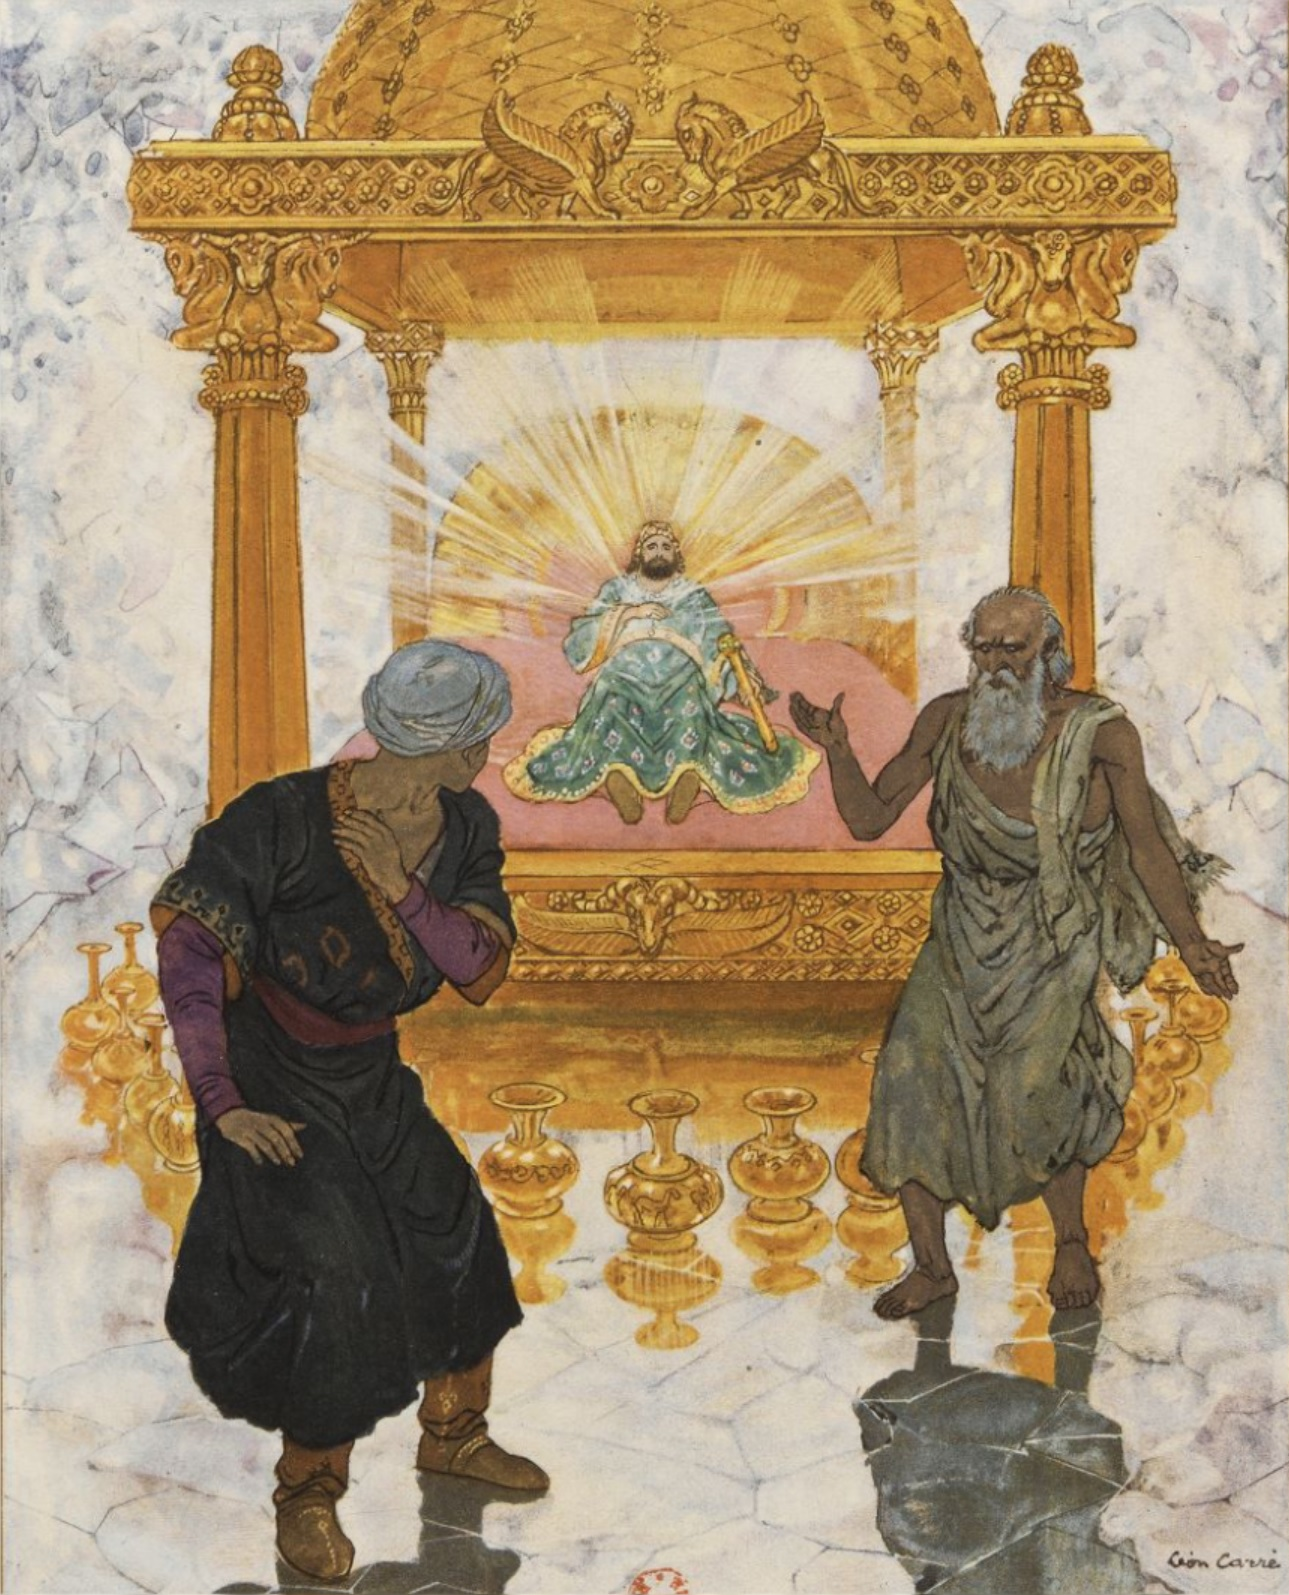
\includegraphics[height=\figsize]{illustrations/volume_4/T04, n0360 - Histoire de la reine Yamlika.jpg}
\end{figure}

\textit{\\
"Ils marchaient ainsi, en s’émerveillant, et commençaient à se demander si la grotte avait une fin, quand ils arrivèrent tout à coup dans une salle immense creusée dans le diamant et qui avait en son milieu un grand lit d’or massif sur lequel était étendu Soleïmân ben-Daoud..."} \\
—T04, n0360 - Histoire de la reine Yamlika \\~\\
\textit{"They walked on and on, marvelling all the time, and suddenly, just as they had begun to wonder whether the cave had any end, turned into a vast hall hewn from the solid diamond, having in its centre a great bed of heavy gold on which lay Sulaiman ibn Daud"} \\
—V02, n0360 - The tale of Yamlika

\newpage

\section{n0375}
\textbf{\Large{The flowering terrace of wit [The youth and his master]}} \\

\begin{figure}[ht]
\centering
\includegraphics[height=\figsize]{illustrations/volume_4/T04, n0375 - Le parterre fleuri de l'esprit [Le jouvenceau et son maître].jpg}
\end{figure}

\textit{\\
"Ils s’assirent donc sur la natte blanche, au clair de lune, et, l’inspiration aidant et la sérénité d’une belle nuit, ils se mi- rent à chanter et à boire, tandis que les doux rayons de l’astre les illuminaient jusqu’à l’extase."} \\
—T04, n0375 - Le parterre fleuri de l'esprit [Le jouvenceau et son maître] \\~\\
\textit{"They sat down on a white mat in the moonlight and began to drink and sing together, the clear night aiding and inspiring them and the stars' soft rays lighting them on to ecstasy."} \\
—V02, n0375 - The flowering terrace of wit [The youth and his master]

\newpage

\section{n0380}
\textbf{\Large{The flowering terrace of wit [The ass]}} \\

\begin{figure}[ht]
\centering
\includegraphics[height=\figsize]{illustrations/volume_4/T04, n0380 - Le parterre fleuri de l'esprit [L'âne].jpg}
\end{figure}

\textit{\\
"Il s’approcha alors de l’homme par derrière, et, tout doucement, défit le licou de l’âne, se le passa à lui-même, sans que l’homme se fût aperçu du changement, et marcha comme une bête de somme, tandis que son compagnon s’éloignait avec l’âne mis en liberté."} \\
—T04, n0380 - Le parterre fleuri de l'esprit [L'âne] \\~\\
\textit{"He went up behind the man and, softly untying the halter from the ass, put it round his own neck, without the exchange being noticed; then he walked along like a beast of burden, while his companion made off with the ass."} \\
—V02, n0380 - The flowering terrace of wit [The ass]

\newpage

\section{n0394}
\textbf{\Large{The strange Khalifah}} \\

\begin{figure}[ht]
\centering
\includegraphics[height=\figsize]{illustrations/volume_4/T04, n0394 - L'étrange Khalifat.jpg}
\end{figure}

\textit{\\
"...ils virent s’approcher le bateau éclairé par la lueur des torches et des flambeaux qu’alimentaient, avec du bois d’aloès, de jeunes esclaves vêtus de satin rouge, les épaules couvertes de manteaux jaunes et la tête enveloppée de mousseline blanche."} \\
—T04, n0394 - L'étrange Khalifat \\~\\
\textit{"...the boat drew near, lighted by torches and cressets, which little slaves dressed in red satin, their shoulders covered with yellow mantles, their heads turbaned with white muslin, fed, from minute to minute, with aloe-wood."} \\
—V02, n0394 - The strange Khalifah

\newpage

\section{n0397}
\textbf{\Large{The strange Khalifah}} \\

\begin{figure}[ht]
\centering
\includegraphics[height=\figsize]{illustrations/volume_4/T04, n0397 - L'étrange Khalifat.jpg}
\end{figure}

\textit{\\
"...un grand rideau au fond fut soulevé, et quatre jeunes esclaves s’avancèrent portant un trône d’or où était assise l’adolescente, avec un visage beau comme un rond de lune, et le collier au cou."} \\
—T04, n0397 - L'étrange Khalifat \\~\\
\textit{"Hardly had I reached the reception hall, when a curtain at the end of it was lifted and four young slaves came towards me, bearing a gold throne on which the girl was seated, wearing the collar on the moonlight of her neck."} \\
—V02, n0397 - The strange Khalifah

\newpage

\section{n0406}
\textbf{\Large{The tale of Rose-in-the-Bud and World’s-Delight}} \\

\begin{figure}[ht]
\centering
\includegraphics[height=\figsize]{illustrations/volume_4/T04, n0406 - Histoire de Rose-dans-le-Calice et de Délice-du-Monde.jpg}
\end{figure}

\textit{\\
"Descends ramasser une quantité de ces courges desséchées, attache-les à ce filet, et jette le tout à la mer. Toi, ne manque point de monter dessus, et alors laisse le courant te porter vers la haute mer, et il te fera parvenir au but que tu souhaites."} \\
—T04, n0406 - Histoire de Rose-dans-le-Calice et de Délice-du-Monde \\~\\
\textit{"Go down and fill this net with dry gourds; then throw all into the sea and climb on top; the current will bear you out and carry you to the place where you would be."} \\
—V02, n0406 - The tale of Rose-in-the-Bud and World’s-Delight

\newpage

\section{n0409}
\textbf{\Large{The tale of Rose-in-the-Bud and World’s-Delight}} \\

\begin{figure}[ht]
\centering
\includegraphics[height=\figsize]{illustrations/volume_4/T04, n0409 - Histoire de Rose-dans-le-Calice et de Délice-du-Monde.jpg}
\end{figure}

\textit{\\
"...au moment où la barque du pêcheur abor- dait, le roi de la ville, dont le nom était le roi Derbas, était assis avec son fils dans son palais à une fenêtre qui donnait sur la mer..."} \\
—T04, n0409 - Histoire de Rose-dans-le-Calice et de Délice-du-Monde \\~\\
\textit{"As the fisherman's boat came to ground, the King of that city, whose name was Dirbas, was sitting with his son at a window in his palace and looking out to sea."} \\
—V02, n0409 - The tale of Rose-in-the-Bud and World’s-Delight

\newpage

\section{n0414}
\textbf{\Large{The magic tale of the ebony horse}} \\

\begin{figure}[ht]
\centering
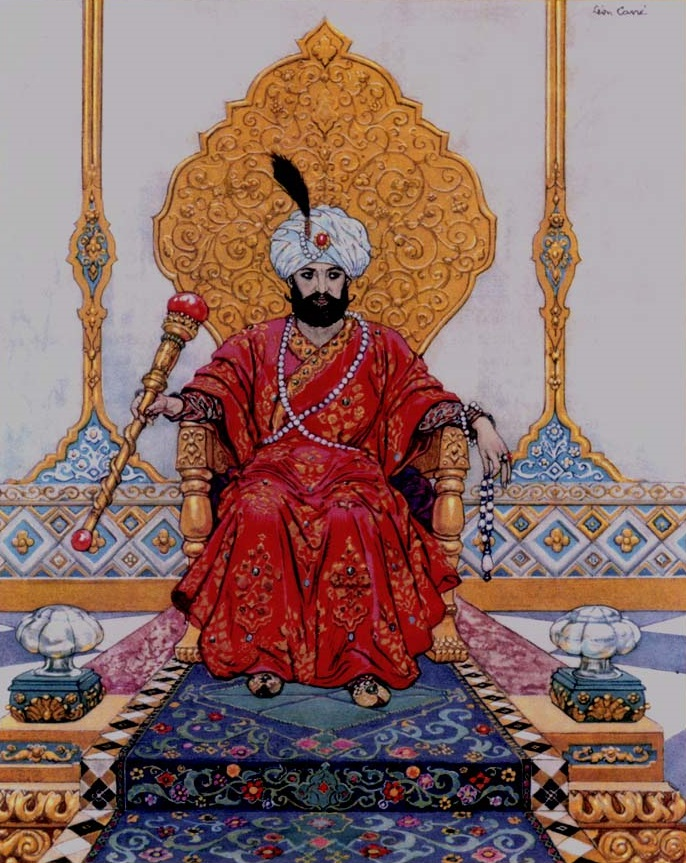
\includegraphics[height=\figsize]{illustrations/volume_4/T04, n0414 - Histoire magique du cheval d'ébène.jpg}
\end{figure}

\textit{\\
"...il y avait dans l’antiquité du temps et le passé des époques et des âges, un roi très grand et très puissant d’entre les rois des Persans, nommé Sabour..."} \\
—T04, n0414 - Histoire magique du cheval d'ébène \\~\\
\textit{"...there was once, in the antiquity of time and the passage of the ages, a great and powerful King of the Persians whose name was Sabur."} \\
—V02, n0414 - The magic tale of the ebony horse

\newpage

\section{n0422}
\textbf{\Large{The magic tale of the ebony horse}} \\

\begin{figure}[ht]
\centering
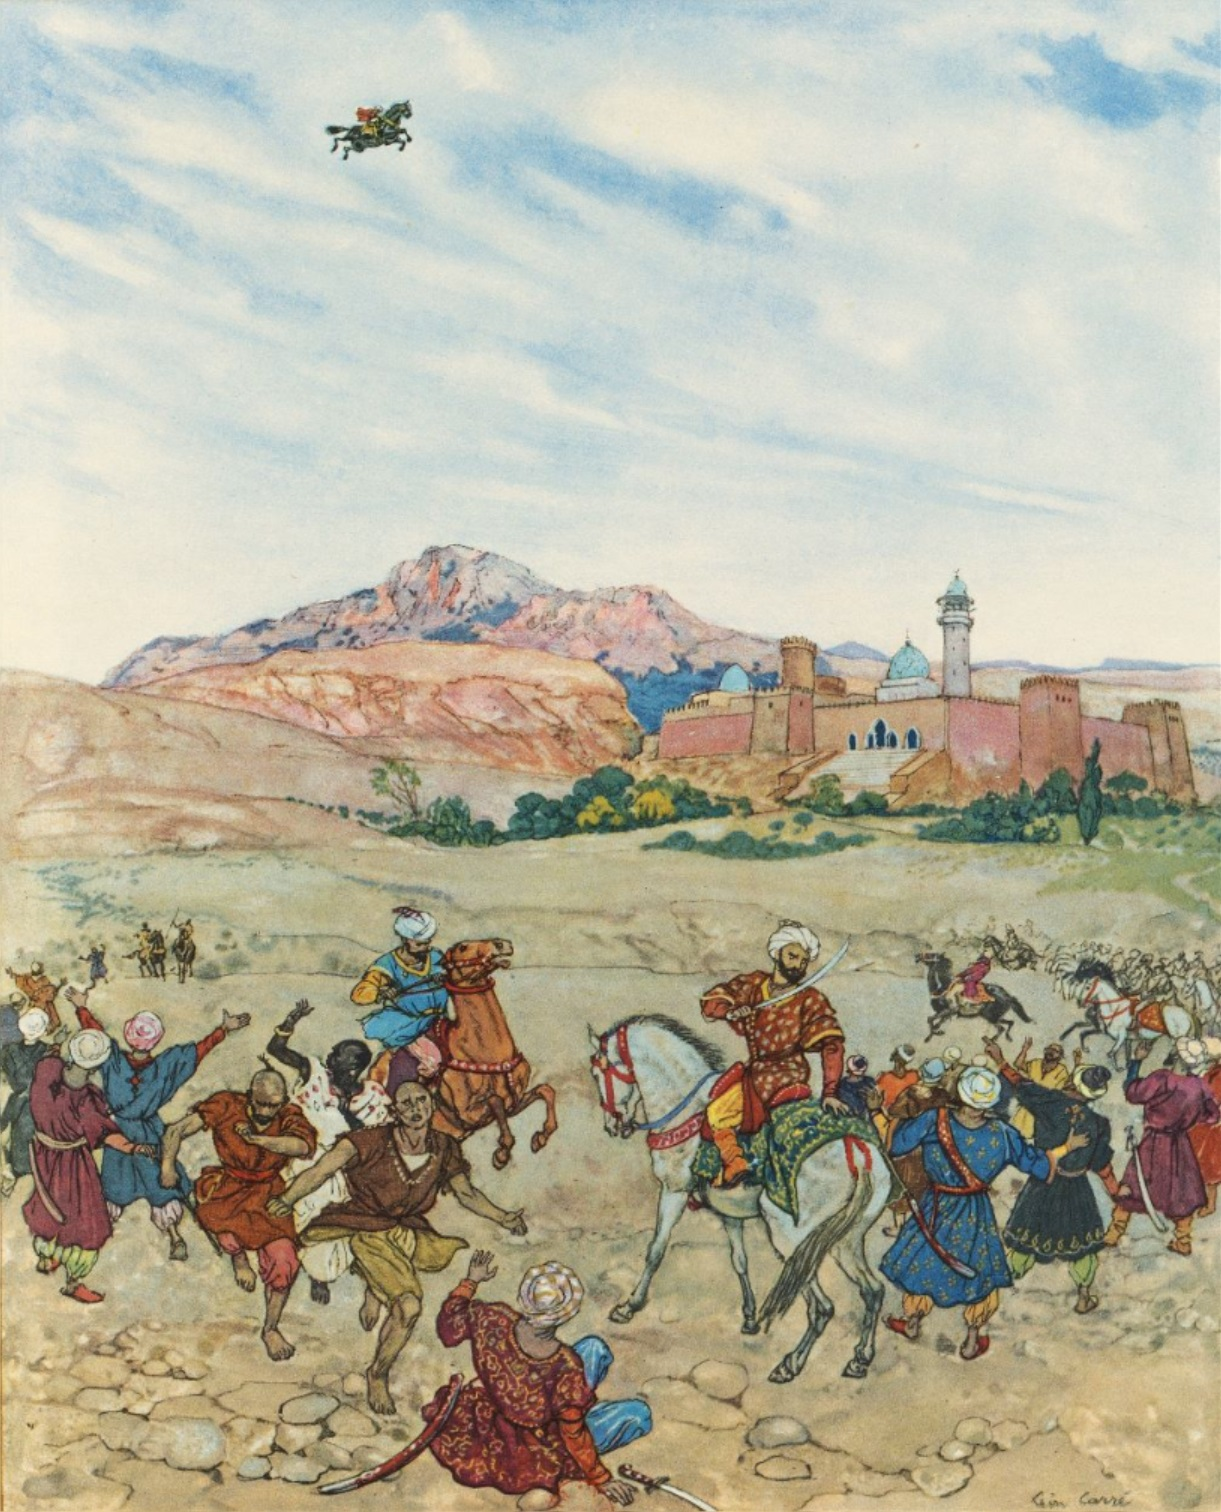
\includegraphics[height=\figsize]{illustrations/volume_4/T04, n0422 - Histoire magique du cheval d'ébène.jpg}
\end{figure}

\textit{\\
"...soudain ses flancs frémirent et se gonflèrent de vent, et, plus rapidement qu’une flèche lancée dans les airs, il prit son essor en s’élevant avec son cavalier en ligne droite dans le ciel !"} \\
—T04, n0422 - Histoire magique du cheval d'ébène \\~\\
\textit{"Suddenly its flanks expanded with the wind and it darted straight up into the sky more quickly than an arrow, carrying its rider with it."} \\
—V02, n0422 - The magic tale of the ebony horse

\newpage

\section{n0433}
\textbf{\Large{The tale of the shifts of Delilah-the-wily}} \\

\begin{figure}[ht]
\centering
\includegraphics[height=\figsize]{illustrations/volume_4/T04, n0433 - Histoire des artifices de Dalila-la-Rouée.jpg}
\end{figure}

\textit{\\
"...elle vit soudain la jeune épouse de l’émir accoudée à sa fenêtre, telle une nouvelle mariée, si belle ! et brillante comme un vrai trésor de tous les bijoux dont elle était ornée, et lumineuse comme une coupole de cristal des blancs habits de neige dont elle était vêtue !"} \\
—T04, n0433 - Histoire des artifices de Dalila-la-Rouée \\~\\
\textit{"...she saw the amir's young wife sitting at her window, seeming a new-married bride because of the great treasure of jewels which she wore, and shining like a dome of crystal in her white expensive clothes."} \\
—V02, n0433 - The tale of the shifts of Delilah-the-wily

\newpage

\section{n0437}
\textbf{\Large{The tale of the shifts of Delilah-the-wily}} \\

\begin{figure}[ht]
\centering
\includegraphics[height=\figsize]{illustrations/volume_4/T04, n0437 - Histoire des artifices de Dalila-la-Rouée.jpg}
\end{figure}

\textit{\\
"...la vieille le quitta et, après avoir tout chargé sur l’âne, se dirigea vers sa maison, en conduisant l’âne par le licou."} \\
—T04, n0437 - Histoire des artifices de Dalila-la-Rouée \\~\\
\textit{"...the old woman loaded all her thefts upon the ass and led it along by its halter in the direction of her house."} \\
—V02, n0437 - The tale of the shifts of Delilah-the-wily

\newpage

\section{n0466}
\textbf{\Large{The tale of Judar the fisherman}} \\

\begin{figure}[ht]
\centering
\includegraphics[height=\figsize]{illustrations/volume_4/T04, n0466 - Histoire de Jouder le pêcheur.jpg}
\end{figure}

\textit{\\
"...lui, pour gagner leur nourriture, se procura un filet de pêche et se mit à aller tous les jours pêcher soit dans le Nil à Boulak..."} \\
—T04, n0466 - Histoire de Jouder le pêcheur \\~\\
\textit{"To earn their living, he bought a fishing-net and went every day to cast it in the Nile at Bulak..."} \\
—V02, n0466 - The tale of Judar the fisherman

\newpage

\section{n0470}
\textbf{\Large{The tale of Judar the fisherman}} \\

\begin{figure}[ht]
\centering
\includegraphics[height=\figsize]{illustrations/volume_4/T04, n0470 - Histoire de Jouder le pêcheur.jpg}
\end{figure}

\textit{\\
"...Jouder monta derrière le Moghrabin sur le dos de la mule, et voyagea de la sorte depuis midi jusqu’au milieu de l’après-midi."} \\
—T04, n0470 - Histoire de Jouder le pêcheur \\~\\
\textit{"...the Moor took Judar up behind him on the mule and they rode from noon until late in the day."} \\
—V02, n0470 - The tale of Judar the fisherman

\end{document}